\chapter{Lagrangiaanse mechanica}\label{ch:b3:lagrangian-mechanics}

Probeer de wet van Newton op te schrijven voor een dubbele slinger: twee
spankrachten, geen van beide vooraf bekend, beide op elk ogenblik van
richting veranderend, en vier scalaire vergelijkingen om te ontwarren,
alleen al om te weten hoe twee hoeken evolueren. Doe nu hetzelfde voor
een kraal op een draaiende hoepel, een keten van gekoppelde veren, een
robotarm. De krachten die een stelsel bijeenhouden --- staven, rails,
scharnieren --- verrichten geen arbeid, en toch dwingt de methode van
Newton ons ze door elke berekening mee te slepen. Dit hoofdstuk
presenteert de herformulering die Lagrange in 1788 publiceerde: beschrijf
het stelsel met de weinige coördinaten die werkelijk kunnen veranderen,
schrijf één enkele functie $L = E_k - E_p$ op, en één recept levert de
bewegingsvergelijkingen in willekeurige coördinaten, met elke staaf en
elke rail al weggewerkt. Beter nog, de nieuwe formulering maakt zichtbaar
wat die van Newton verbergt: elke symmetrie van $L$ levert een behouden
grootheid --- de impuls uit de homogeniteit van de ruimte, de energie uit
die van de tijd --- een resultaat van Emmy Noether dat ver buiten de
mechanica het ordenende beginsel van de natuurkunde is geworden.

\section{Van krachten naar coördinaten}

\begin{definition}[Dwangvoorwaarden, vrijheidsgraden, gegeneraliseerde coördinaten]\label{def:b3:lagrangian-mechanics:coordinates}
\index{dwangvoorwaarde}\index{vrijheidsgraden}\index{gegeneraliseerde coördinaten}
Een \emph{dwangvoorwaarde} is een meetkundige voorwaarde die aan de
posities van een stelsel wordt opgelegd --- een kraal blijft op zijn
draad, de staaf van een slinger houdt een vaste lengte, twee wielen van
één as draaien samen. Een dwangvoorwaarde die als een vergelijking
$f(\vect r_1, \dots, \vect r_N, t) = 0$ tussen de coördinaten (en
eventueel de tijd) te schrijven is, heet \emph{holonoom}. Het aantal
onafhankelijke manieren waarop de configuratie nog kan variëren is het
aantal \emph{vrijheidsgraden} $n$; elk stel van $n$ onafhankelijke
grootheden $q_1, \dots, q_n$ dat de configuratie volledig vastlegt is een
stel \emph{gegeneraliseerde coördinaten} --- hoeken, lengten of een
willekeurige handige mengeling. Hun tijdsafgeleiden
$\dot q_1, \dots, \dot q_n$ heten de \emph{gegeneraliseerde snelheden}\index{gegeneraliseerde snelheden}.
\end{definition}

\begin{example}[Vrijheidsgraden tellen]\label{ex:b3:lagrangian-mechanics:counting}
Een punt op een tafel: $n = 2$. Een vlakke slinger met vaste lengte: één
hoek, $n = 1$. Een dubbele slinger: twee hoeken, $n = 1 + 1 = 2$. Een
kraal op een starre hoepel: één hoek, $n = 1$ --- ook wanneer de hoepel
zelf gedwongen wordt te draaien, want de opgelegde rotatie voegt geen
vrijheid toe. Een star lichaam dat vrij in de ruimte beweegt: drie
coördinaten van zijn zwaartepunt plus drie hoeken, $n = 6$. Een gas van
$N$ vrije moleculen (punten): $n = 3N$. Elke holonome \omterm{def:b3:lagrangian-mechanics:coordinates}{dwangvoorwaarde}
neemt één vrijheidsgraad weg: twee punten verbonden door een staaf hebben
$3 + 3 - 1 = 5$.
\end{example}

\begin{omfigure}
\begin{tikzpicture}[font=\small, >=Stealth]
  % (a) plane pendulum
  \begin{scope}
    \draw[thick] (-1,0) -- (1,0);
    \foreach \i in {-0.8,-0.5,-0.2,0.1,0.4,0.7} \draw (\i,0) -- (\i+0.18,0.16);
    \fill (0,0) circle (1.5pt);
    \draw[dashed] (0,0) -- (0,-2.2);
    \draw[thick] (0,0) -- (-55:2.1);
    \fill[omDef] (-55:2.1) circle (3pt);
    \draw[->] (0,-1.0) arc (-90:-55:1.0);
    \node at (-72:1.35) {$\theta$};
    \node at (-55:2.5) {$m$};
    \node at ($(-55:1.35)+(0.28,0.12)$) {$\ell$};
    \node at (0,-2.9) {één coördinaat: $\theta$};
  \end{scope}
  % (b) bead on rotating hoop
  \begin{scope}[xshift=6.2cm]
    \coordinate (C) at (0,-2.35);
    \draw[thick] (C) circle (1.55);
    \draw[dashed] (0,-0.3) -- (0,-4.6);
    \draw[->, thick] (0.35,-0.15) arc (20:160:0.37);
    \node at (0,0.25) {$\omega$};
    \fill (C) circle (1pt);
    \draw (C) -- ++(-50:1.55);
    \fill[omDef] ($(C)+(-50:1.55)$) circle (3pt);
    \draw[->] ($(C)+(0,-0.85)$) arc (-90:-50:0.85);
    \node at ($(C)+(-70:1.18)$) {$\theta$};
    \node at ($(C)+(-38:2.0)$) {$m$};
    \draw (C) -- ++(135:1.55);
    \node at (-1.35,-1.35) {$R$};
    \node at (0,-4.95) {één coördinaat: $\theta$};
  \end{scope}
  % (c) double pendulum
  \begin{scope}[xshift=11.4cm]
    \draw[thick] (-0.9,0) -- (0.9,0);
    \foreach \i in {-0.7,-0.4,-0.1,0.2,0.5} \draw (\i,0) -- (\i+0.18,0.16);
    \fill (0,0) circle (1.5pt);
    \draw[dashed] (0,0) -- (0,-1.7);
    \draw[thick] (0,0) -- (-65:1.5) coordinate (m1);
    \fill[omDef] (m1) circle (2.6pt);
    \draw[dashed] (m1) -- ++(0,-1.5);
    \draw[thick] (m1) -- ++(-40:1.5) coordinate (m2);
    \fill[omThm] (m2) circle (2.6pt);
    \draw[->] (0,-0.8) arc (-90:-65:0.8);
    \node at (-80:1.1) {$\theta_1$};
    \draw[->] ($(m1)+(0,-0.75)$) arc (-90:-40:0.75);
    \node at ($(m1)+(-68:1.05)$) {$\theta_2$};
    \node at (0.3,-3.4) {twee coördinaten: $\theta_1, \theta_2$};
  \end{scope}
\end{tikzpicture}

{\small \omterm{def:b3:lagrangian-mechanics:coordinates}{Gegeneraliseerde coördinaten}: elk stelsel wordt beschreven door de
hoeken die werkelijk kunnen veranderen, niet door de cartesische
coördinaten van zijn massa's. De spankrachten in de staven en de
normaalkracht van de hoepel komen er nooit in voor.}
\end{omfigure}

\section{Het beginsel van de kleinste actie}

\begin{definition}[Lagrangiaan en actie]\label{def:b3:lagrangian-mechanics:action}
\index{lagrangiaan}\index{actie}
De \emph{lagrangiaan} van een mechanisch stelsel waarvan de krachten
afleidbaar zijn uit een potentiële energie $E_p$ is de functie van de
coördinaten, de snelheden en eventueel de tijd
\[
L(q, \dot q, t) = E_k - E_p ,
\]
de kinetische energie \emph{min} de potentiële, beide uitgedrukt in de
\omterm{def:b3:lagrangian-mechanics:coordinates}{gegeneraliseerde coördinaten}. De \emph{actie} van een denkbare beweging
$q(t)$ tussen vaste eindpunten $q(t_1)$ en $q(t_2)$ is het getal
\[
S[q] = \int_{t_1}^{t_2} L\big(q(t), \dot q(t), t\big)\,\dd t .
\]
$S$ is een \emph{functionaal}: hij verslindt een heel pad en geeft één
getal terug, in joulesecondes --- de eenheid van de constante van Planck.
\end{definition}

\begin{theorem}[Beginsel van Hamilton en de vergelijkingen van Euler--Lagrange]\label{thm:b3:lagrangian-mechanics:euler-lagrange}
\index{beginsel van Hamilton}\index{vergelijkingen van Euler--Lagrange}\index{kleinste actie}
Van alle denkbare bewegingen die dezelfde twee eindpunten in dezelfde tijd
verbinden, is de werkelijke beweging die welke de \omterm{def:b3:lagrangian-mechanics:action}{actie}
\emph{stationair} maakt (het \emph{\omterm{thm:b3:lagrangian-mechanics:euler-lagrange}{beginsel van Hamilton}}, of het beginsel
van de \emph{\omterm{thm:b3:lagrangian-mechanics:euler-lagrange}{kleinste actie}}). Gelijkwaardig: de beweging voldoet aan de
\emph{\omterm{thm:b3:lagrangian-mechanics:euler-lagrange}{vergelijkingen van Euler--Lagrange}}
\[
\frac{\dd}{\dd t}\frac{\partial L}{\partial\dot q_i}
 - \frac{\partial L}{\partial q_i} = 0 ,
\qquad i = 1, \dots, n :
\]
één tweede-ordevergelijking per vrijheidsgraad, in welke coördinaten dan
ook gekozen zijn.
\end{theorem}

\begin{proof}
Vervorm het pad: $q_i(t) \to q_i(t) + \delta q_i(t)$ met
$\delta q_i(t_1) = \delta q_i(t_2) = 0$. Tot op eerste orde geldt
\[
\delta S = \int_{t_1}^{t_2}\sum_i\Big(
  \frac{\partial L}{\partial q_i}\,\delta q_i
 + \frac{\partial L}{\partial\dot q_i}\,\delta\dot q_i\Big)\dd t
 = \int_{t_1}^{t_2}\sum_i\Big(
  \frac{\partial L}{\partial q_i}
 - \frac{\dd}{\dd t}\frac{\partial L}{\partial\dot q_i}\Big)\delta q_i\,\dd t ,
\]
na partiële integratie van de tweede term ($\delta\dot q_i =
\dd(\delta q_i)/\dd t$) en het weglaten van de randterm, die op de vaste
eindpunten verdwijnt. Is $\delta S = 0$ voor \emph{elke} vervorming, dan
moet het haakje op elk ogenblik en voor elke $i$ nul zijn --- was het
ergens positief, dan gaf een daar geconcentreerde bult $\delta q_i$ een
$\delta S \neq 0$. Het omgekeerde leest men van dezelfde regel af.
\end{proof}

\begin{omfigure}
\begin{tikzpicture}[font=\small, >=Stealth]
  \draw[->] (0,0) -- (7.6,0) node[right] {$t$};
  \draw[->] (0,0) -- (0,3.4) node[above] {$q$};
  \fill (0.8,0.7) circle (2pt) node[below left] {$q(t_1)$};
  \fill (6.8,2.3) circle (2pt) node[above right] {$q(t_2)$};
  \draw[omDef, very thick] (0.8,0.7) .. controls (2.6,2.6) and (5.0,1.4) .. (6.8,2.3);
  \draw[omExo, dashed] (0.8,0.7) .. controls (2.2,0.6) and (5.4,0.9) .. (6.8,2.3);
  \draw[omExo, dashed] (0.8,0.7) .. controls (3.0,3.6) and (5.2,2.9) .. (6.8,2.3);
  \node[omDef] at (1.9,3.35) {werkelijk pad};
  \draw[->, omDef] (2.25,3.15) -- (2.85,2.3);
  \node[omExo] at (3.4,0.42) {gevarieerde paden};
  \draw[<->] (4.1,1.62) -- (4.1,2.62);
  \node at (4.55,2.15) {$\delta q$};
\end{tikzpicture}

{\small Het \omterm{thm:b3:lagrangian-mechanics:euler-lagrange}{beginsel van Hamilton}: van alle paden met dezelfde eindpunten
en dezelfde duur maakt het werkelijke pad $S = \int L\,\dd t$ stationair
--- vervormingen $\delta q$ van eerste orde veranderen $S$ pas in tweede
orde.}
\end{omfigure}

\begin{proposition}[Newton teruggevonden]\label{prop:b3:lagrangian-mechanics:newton}
Voor een deeltje in cartesische coördinaten is $L = \tfrac12 m(\dot x^2 +
\dot y^2 + \dot z^2) - E_p(x,y,z)$, en de \omterm{thm:b3:lagrangian-mechanics:euler-lagrange}{vergelijkingen van
Euler--Lagrange} luiden $m\ddot x = -\partial E_p/\partial x$ en zo ook
voor $y$ en $z$: precies $m\vect a = \vect F$. De lagrangiaanse en de
newtoniaanse mechanica stemmen overeen waar beide gelden; de nieuwe vorm
overleeft eenvoudigweg een verandering van coördinaten, wat Newtons
componentvergelijkingen niet doen.
\end{proposition}

\begin{proof}
$\partial L/\partial\dot x = m\dot x$, $\partial L/\partial x =
-\partial E_p/\partial x$; de vergelijking van Euler--Lagrange luidt
$\dd(m\dot x)/\dd t + \partial E_p/\partial x = 0$.
\end{proof}

\begin{remark}[Waarom de dwangkrachten verdwijnen]\label{rem:b3:lagrangian-mechanics:constraints}
De spankracht van een staaf, de normaalkracht van een rail, staan loodrecht
op elke verplaatsing die de \omterm{def:b3:lagrangian-mechanics:coordinates}{dwangvoorwaarde} toelaat: zij verrichten geen
arbeid in enige beweging die met de voorwaarde verenigbaar is. Omdat de
\omterm{def:b3:lagrangian-mechanics:action}{actie} is opgebouwd uit energieën die alleen op zulke bewegingen worden
geëvalueerd, komen deze krachten nooit in $L$ voor --- dat is het
praktische wonder van de methode. De algemene rechtvaardiging (het
beginsel van de virtuele arbeid van d'Alembert) wordt hier aangenomen;
voor elk stelsel in dit boek kan het recept hieronder rechtstreeks tegen
Newton worden getoetst, zoals \cref{prop:b3:lagrangian-mechanics:newton}
begon te doen. Wil men een dwangkracht zelf kennen --- knapt de staaf? ---
dan keert men voor die ene kracht naar Newton terug, met de beweging al
bekend.
\end{remark}

\begin{method}[Het lagrangiaanse recept]\label{met:b3:lagrangian-mechanics:recipe}
(1) Tel de \omterm{def:b3:lagrangian-mechanics:coordinates}{vrijheidsgraden} en kies coördinaten $q_i$ --- hoeken voor
rotaties, abscissen langs rails. (2) Druk de posities $\vect r(q_i, t)$
uit, differentieer naar de tijd om de snelheden te krijgen en schrijf
$E_k$; schrijf $E_p$. (3) $L = E_k - E_p$, waarbij elke additieve
constante mag vervallen. (4) Eén vergelijking van Euler--Lagrange per
coördinaat. (5) Oogst vóór het oplossen de behouden grootheden: cyclische
coördinaten (\cref{def:b3:lagrangian-mechanics:momentum}) en de
\omterm{prop:b3:lagrangian-mechanics:energy}{energiefunctie} (\cref{prop:b3:lagrangian-mechanics:energy}). (6) Toets de
limieten: kleine hoeken, uitgeschakelde rotatie, bekende bijzondere
gevallen.
\end{method}

\begin{example}[De slinger, in drie regels]\label{ex:b3:lagrangian-mechanics:pendulum}
Eén coördinaat $\theta$; $\vect v = \ell\dot\theta\,\vect e_\theta$, dus
$E_k = \tfrac12 m\ell^2\dot\theta^2$ en $E_p = -mg\ell\cos\theta$. Dan is
$L = \tfrac12 m\ell^2\dot\theta^2 + mg\ell\cos\theta$, en
$\dd(m\ell^2\dot\theta)/\dd t = -mg\ell\sin\theta$:
\[
\ddot\theta = -\frac{g}{\ell}\sin\theta ,
\]
de vergelijking die het volume van jaar 1 uit het moment van de
zwaartekracht verkreeg --- met de spankracht nooit genoemd.
\end{example}

\begin{example}[Kraal op een draaiende hoepel]\label{ex:b3:lagrangian-mechanics:hoop}
Een kraal met massa $m$ glijdt op een verticale cirkelvormige hoepel met
straal $R$ die gedwongen wordt met constante $\omega$ om zijn verticale
middellijn te draaien (\cref{ex:b3:lagrangian-mechanics:counting}). Eén
coördinaat, de poolhoek $\theta$ vanaf het laagste punt. De snelheid van
de kraal heeft een component $R\dot\theta$ langs de hoepel en, loodrecht
daarop, een component $\omega R\sin\theta$ door de opgelegde rotatie:
\[
L = \tfrac12 mR^2\dot\theta^2 + \tfrac12 m\omega^2R^2\sin^2\theta
 + mgR\cos\theta ,
\qquad
mR^2\ddot\theta = m\omega^2R^2\sin\theta\cos\theta - mgR\sin\theta .
\]
Evenwichten waar $\ddot\theta = 0$: het laagste punt $\theta = 0$ (en het
hoogste, altijd onstabiel), en, zodra $\omega^2 > g/R$, een nieuw paar
$\cos\theta_{\text{eq}} = g/\omega^2R$. Schrijven we de vergelijking als
$mR^2\ddot\theta = -\dd U_{\text{eff}}/\dd\theta$ met de \emph{effectieve
potentiële energie}\index{effectieve potentiële energie}
\[
U_{\text{eff}}(\theta) = -mgR\cos\theta
 - \tfrac12 m\omega^2R^2\sin^2\theta
\]
dan wordt de meetkunde zichtbaar: onder de kritische draaisnelheid
$\omega_{\text{c}} = \sqrt{g/R}$ is het laagste punt een put; erboven
wordt het een top en gaat de kraal op de helling liggen, steeds hoger
naarmate de hoepel sneller draait --- het beginsel van de
centrifugaalregulateur die stoommachines regelde.
\end{example}

\begin{omfigure}
\begin{tikzpicture}
  \begin{axis}[omaxis, axis x line=bottom, axis y line=left,
    width=11.4cm, height=5.6cm, xmin=-180, xmax=180,
    ymin=-1.65, ymax=1.2, xlabel={$\theta$ (graden)},
    xlabel style={at={(axis description cs:0.5,-0.1)}, anchor=north},
    ylabel={$U_{\text{eff}}/mgR$}, xtick={-180,-90,0,90,180}, ytick=\empty,
    clip=false,
    legend style={font=\scriptsize, at={(0.5,-0.32)}, anchor=north,
      draw=none, fill=none, legend columns=2}]
    \addplot[omDef, thick, domain=-180:180, samples=90]
      {-cos(x) - 0.25*sin(x)^2};
    \addlegendentry{$\omega^2 = g/2R$ (traag): put bij $\theta = 0$}
    \addplot[omThm, thick, domain=-180:180, samples=90]
      {-cos(x) - 1.0*sin(x)^2};
    \addlegendentry{$\omega^2 = 2g/R$ (snel): putten bij $\pm 60^\circ$}
    \fill[omThm] (axis cs:60,-1.25) circle (1.8pt);
    \fill[omThm] (axis cs:-60,-1.25) circle (1.8pt);
    \fill[omDef] (axis cs:0,-1) circle (1.8pt);
  \end{axis}
\end{tikzpicture}

{\small De effectieve potentiaal van de kraal op de draaiende hoepel.
Zodra $\omega$ de waarde $\sqrt{g/R}$ passeert, splitst de enkele put
onderaan in twee symmetrische putten: de evenwichtshoek stijgt met de
draaisnelheid.}
\end{omfigure}

\section{Symmetrieën en behoudswetten}

\begin{definition}[Gegeneraliseerde impuls, cyclische coördinaat]\label{def:b3:lagrangian-mechanics:momentum}
\index{gegeneraliseerde impuls}\index{cyclische coördinaat}
De \emph{gegeneraliseerde impuls} geconjugeerd aan de coördinaat $q_i$ is
\[
p_i = \frac{\partial L}{\partial\dot q_i} .
\]
Voor een cartesische coördinaat is dat de gewone impuls $m\dot x$; voor
een hoek is het een impulsmoment. Een coördinaat die niet in $L$ voorkomt
(al komt haar snelheid er wel in voor) heet \emph{cyclisch}.
\end{definition}

\begin{proposition}[Cyclische coördinaten geven behoudswetten]\label{prop:b3:lagrangian-mechanics:cyclic}
Is $q_i$ cyclisch, dan blijft de geconjugeerde impuls behouden:
$\partial L/\partial q_i = 0$ geeft $\dd p_i/\dd t = 0$. Coördinaten zó
kiezen dat er zo veel mogelijk cyclisch zijn is de meest doeltreffende
stap bij het oplossen van een mechanicavraagstuk.
\end{proposition}

\begin{proof}
Onmiddellijk uit de vergelijking van Euler--Lagrange voor $q_i$.
\end{proof}

\begin{example}[Centrale kracht, opgelost door kijken]\label{ex:b3:lagrangian-mechanics:central}
Een deeltje in een centrale potentiaal $E_p(r)$, in poolcoördinaten in
zijn bewegingsvlak:
\[
L = \tfrac12 m(\dot r^2 + r^2\dot\varphi^2) - E_p(r) .
\]
$\varphi$ is cyclisch, dus $p_\varphi = mr^2\dot\varphi$ --- het
impulsmoment --- blijft behouden: de perkenwet van Kepler, die het volume
van jaar 1 uit de momentvergelijking afleidde, valt hier vanzelf uit vóór
er ook maar één vergelijking is opgelost. De overblijvende radiale
vergelijking is $m\ddot r = mr\dot\varphi^2 - E_p'(r)$, dat wil zeggen de
eendimensionale beweging in de effectieve potentiaal $E_p(r) + p_\varphi^2/2mr^2$ van dat volume.
\end{example}

\begin{theorem}[Stelling van Noether]\label{thm:b3:lagrangian-mechanics:noether}
\index{stelling van Noether}\index{symmetrie}
Bij elke continue symmetrie van de \omterm{def:b3:lagrangian-mechanics:action}{lagrangiaan} hoort een behouden
grootheid. Nauwkeurig: laat de verschuiving $q_i \to q_i + \varepsilon\,K_i(q)$ de $L$ tot op eerste orde in $\varepsilon$
onveranderd voor alle bewegingen, dan is
\[
Q = \sum_i p_i\,K_i(q)
\]
constant langs elke werkelijke beweging. De homogeniteit van de ruimte
(invariantie onder translatie) levert de impuls; de isotropie van de
ruimte (invariantie onder rotatie) levert het impulsmoment; de
homogeniteit van de tijd levert de energie
(\cref{prop:b3:lagrangian-mechanics:energy}).
\end{theorem}

\begin{proof}
Invariantie tot op eerste orde betekent
$0 = \delta L = \sum_i\big(\partial_{q_i}L\,K_i +
\partial_{\dot q_i}L\,\dot K_i\big)\varepsilon$. Op een werkelijke
beweging is $\partial_{q_i}L = \dot p_i$ volgens Euler--Lagrange, dus het
haakje is $\sum_i(\dot p_iK_i + p_i\dot K_i) = \dd Q/\dd t$. Een \omterm{def:b3:lagrangian-mechanics:momentum}{cyclische
coördinaat} is het bijzondere geval $K_i = \delta_{ij}$. Het geval van de
tijdverschuiving vergt de aparte berekening van
\cref{prop:b3:lagrangian-mechanics:energy}; de volledige stelling, voor
transformaties die ook $t$ veranderen of $L$ met een totale afgeleide
wijzigen, wordt in colleges over analytische mechanica bewezen en hier in
die algemeenheid aangenomen.
\end{proof}

\begin{proposition}[De energiefunctie]\label{prop:b3:lagrangian-mechanics:energy}
\index{energiefunctie}
Langs elke beweging voldoet de \emph{\omterm{prop:b3:lagrangian-mechanics:energy}{energiefunctie}}
\[
h = \sum_i \dot q_i\,\frac{\partial L}{\partial\dot q_i} - L
\qquad\text{aan}\qquad
\frac{\dd h}{\dd t} = -\frac{\partial L}{\partial t} .
\]
Hangt $L$ niet expliciet van de tijd af, dan blijft $h$ behouden. Bevatten
bovendien de betrekkingen $\vect r(q)$ tussen posities en coördinaten de
tijd niet --- geen opgelegde rotatie, geen bewegende ophanging --- dan is
$E_k$ een kwadratische vorm in de $\dot q_i$ en geldt $h = E_k + E_p$: de
mechanische energie. Bij een tijdafhankelijke \omterm{def:b3:lagrangian-mechanics:coordinates}{dwangvoorwaarde} blijft $h$
nog steeds behouden zodra $\partial L/\partial t = 0$, maar het is
\emph{niet} de energie: de motor die de \omterm{def:b3:lagrangian-mechanics:coordinates}{dwangvoorwaarde} afdwingt wisselt
arbeid met het stelsel uit.
\end{proposition}

\begin{proof}
$\dd h/\dd t = \sum_i(\ddot q_ip_i + \dot q_i\dot p_i) -
\sum_i(\partial_{q_i}L\,\dot q_i + \partial_{\dot q_i}L\,\ddot q_i) -
\partial_tL$. De termen in $\ddot q_i$ vallen weg; de \omterm{thm:b3:lagrangian-mechanics:euler-lagrange}{vergelijkingen van
Euler--Lagrange} maken van $\dot p_i$ een $\partial_{q_i}L$, wat het
volgende paar wegstreept; $-\partial_tL$ blijft over. Is $E_k = \tfrac12\sum a_{jk}(q)\dot
q_j\dot q_k$, dan geeft de identiteit van Euler
voor kwadratische vormen $\sum\dot
q_i\,\partial E_k/\partial\dot q_i = 2E_k$, dus $h = 2E_k - (E_k - E_p)
= E_k + E_p$.
\end{proof}

\begin{example}[De draaiende hoepel bewaart $h$, niet $E$]\label{ex:b3:lagrangian-mechanics:hoop-energy}
Voor de kraal van \cref{ex:b3:lagrangian-mechanics:hoop} bevat $L$ geen
expliciete $t$, dus $h = \tfrac12 mR^2\dot\theta^2 + U_{\text{eff}}
(\theta)$ blijft behouden --- maar de mechanische energie $E = \tfrac12
mR^2\dot\theta^2 + \tfrac12 m\omega^2R^2\sin^2\theta - mgR\cos\theta$ niet:
$E = h + m\omega^2R^2\sin^2\theta$ verandert terwijl de kraal glijdt. Het
verschil is de arbeid van de motor die $\omega$ constant houdt terwijl de
afstand van de kraal tot de as verandert.
\end{example}

\section{Geladen deeltjes en kleine trillingen}

\begin{proposition}[Lagrangiaan van een geladen deeltje]\label{prop:b3:lagrangian-mechanics:charge}
\index{snelheidsafhankelijke potentiaal}
In een elektromagnetisch veld beschreven door de potentialen $V$ en
$\vect A$ (met $\vect E = -\vect\nabla V - \partial_t\vect A$ en
$\vect B = \operatorname{\vect{curl}}\vect A$, zoals in het volume van
jaar 2) levert de \omterm{def:b3:lagrangian-mechanics:action}{lagrangiaan}
\[
L = \tfrac12 m\vect v^{\,2} - qV + q\,\vect v\cdot\vect A
\]
via de \omterm{thm:b3:lagrangian-mechanics:euler-lagrange}{vergelijkingen van Euler--Lagrange} precies de lorentzkracht
$m\dot{\vect v} = q(\vect E + \vect v\wedge\vect B)$. De magnetische
kracht, die geen arbeid verricht en uit geen gewone potentiële energie
volgt, komt binnen via een term lineair in de snelheid; de geconjugeerde
impuls wordt $\vect p = m\vect v + q\vect A$, niet langer $m\vect v$
alleen.
\end{proposition}

\begin{proof}
Voor de $x$-component: $p_x = m\dot x + qA_x$, en
$\partial_xL = -q\,\partial_xV + q\,\vect v\cdot\partial_x\vect A$. De
vergelijking van Euler--Lagrange geeft $m\ddot x = -q\,\partial_xV -
q\,\dd A_x/\dd t + q\,\vect v\cdot\partial_x\vect A$. Langs de beweging is
$\dd A_x/\dd t = \partial_tA_x + (\vect v\cdot\vect\nabla)A_x$, dus
$m\ddot x = qE_x + q\big[\vect v\cdot\partial_x\vect A - (\vect v\cdot
\vect\nabla)A_x\big]$, en het haakje is de $x$-component van $\vect
v\wedge(\vect\nabla\wedge\vect A) = \vect v\wedge\vect B$ --- werk beide
uit ter controle.
\end{proof}

\begin{proposition}[Kleine trillingen en eigentrillingen]\label{prop:b3:lagrangian-mechanics:modes}
\index{eigentrillingen}\index{kleine trillingen}
Nabij een stabiel evenwicht $q^{\text{eq}}$ ontwikkelen we $L$ tot op
tweede orde in de uitwijkingen $u_i = q_i - q_i^{\text{eq}}$:
$L \approx \tfrac12\sum m_{ij}\dot u_i\dot u_j -
\tfrac12\sum k_{ij}u_iu_j$ met constante symmetrische matrices. De
bewegingsvergelijkingen zijn lineair, en elke beweging is een superpositie
van \emph{\omterm{prop:b3:lagrangian-mechanics:modes}{eigentrillingen}}: collectieve trillingen $u_i(t) = a_i\cos(\Omega t
+ \phi)$ waarin alle coördinaten met één gemeenschappelijke frequentie
meebewegen, terwijl de amplitudes en de frequenties voldoen aan
$\sum_j(k_{ij} -
\Omega^2m_{ij})\,a_j = 0$ --- een
eigenwaardevraagstuk voor matrices, met $n$ modi voor $n$
\omterm{def:b3:lagrangian-mechanics:coordinates}{vrijheidsgraden}.
\end{proposition}

\begin{proof}
Lineaire termen verdwijnen in een evenwicht; de \omterm{thm:b3:lagrangian-mechanics:euler-lagrange}{vergelijkingen van
Euler--Lagrange} van de kwadratische $L$ luiden $\sum_jm_{ij}\ddot u_j = -\sum_jk_{ij}u_j$. Invullen van de proeftrilling geeft het genoemde
lineaire stelsel, dat pas een amplitudevector ongelijk nul heeft wanneer
$\det(k_{ij} -
\Omega^2m_{ij}) = 0$: $n$ waarden van $\Omega^2$, alle
positief in een stabiel evenwicht. Dat de algemene beweging een
superpositie van de modi is, is de simultane diagonalisatie van twee
kwadratische vormen, een resultaat uit de lineaire algebra van het
wiskundevolume van jaar 2; de volledigheid wordt aangenomen.
\end{proof}

\begin{example}[Twee slingers gekoppeld door een veer]\label{ex:b3:lagrangian-mechanics:coupled}
Twee gelijke slingers (massa $m$, lengte $\ell$), met hun gewichten
verbonden door een veer met veerconstante $k$ die ontspannen is als beide
recht naar beneden hangen. Voor kleine hoeken geldt
\[
L = \tfrac12 m\ell^2(\dot\theta_1^2 + \dot\theta_2^2)
 - \tfrac12 mg\ell(\theta_1^2 + \theta_2^2)
 - \tfrac12 k\ell^2(\theta_2 - \theta_1)^2 .
\]
De symmetrie suggereert de combinaties $s = \theta_1 + \theta_2$ en $d =
\theta_1 - \theta_2$, die de vergelijkingen ontkoppelen: de \emph{modus in
fase} ($\theta_1 = \theta_2$, veer werkloos) bij $\Omega_1 =
\sqrt{g/\ell}$, en de \emph{modus in tegenfase} ($\theta_1 = -\theta_2$,
veer dubbel gerekt) bij $\Omega_2 = \sqrt{g/\ell + 2k/m}$. Zet één slinger
alleen in beweging --- een gelijke menging van de twee modi --- en de
energie verhuist volledig van de ene slinger naar de andere en terug, met
de zweeffrequentie $(\Omega_2 - \Omega_1)/2\pi$: de demonstratie met
gekoppelde slingers, en het mechanisme achter elke resonante
energieoverdracht, van afgestemde kringen tot moleculaire trillingen.
\end{example}

\begin{omfigure}
\begin{tikzpicture}[font=\small, >=Stealth]
  % in-phase mode
  \begin{scope}
    \draw[thick] (-0.4,0) -- (3.4,0);
    \foreach \i in {-0.2,0.3,0.8,1.3,1.8,2.3,2.8} \draw (\i,0) -- (\i+0.18,0.16);
    \fill (0.5,0) circle (1.2pt);
    \fill (2.5,0) circle (1.2pt);
    \draw[thick] (0.5,0) -- ++(-75:1.9) coordinate (a1);
    \draw[thick] (2.5,0) -- ++(-75:1.9) coordinate (a2);
    \fill[omDef] (a1) circle (2.6pt);
    \fill[omDef] (a2) circle (2.6pt);
    \draw[decorate, decoration={coil, aspect=0.6, segment length=3pt, amplitude=2pt}] (a1) -- (a2);
    \draw[->, omDef] ($(a1)+(0.05,-0.3)$) -- ++(0.5,0);
    \draw[->, omDef] ($(a2)+(0.05,-0.3)$) -- ++(0.5,0);
    \node at (1.5,-2.9) {in fase: $\Omega_1 = \sqrt{g/\ell}$};
  \end{scope}
  % opposed mode
  \begin{scope}[xshift=6.4cm]
    \draw[thick] (-0.4,0) -- (3.4,0);
    \foreach \i in {-0.2,0.3,0.8,1.3,1.8,2.3,2.8} \draw (\i,0) -- (\i+0.18,0.16);
    \fill (0.5,0) circle (1.2pt);
    \fill (2.5,0) circle (1.2pt);
    \draw[thick] (0.5,0) -- ++(-105:1.9) coordinate (b1);
    \draw[thick] (2.5,0) -- ++(-75:1.9) coordinate (b2);
    \fill[omThm] (b1) circle (2.6pt);
    \fill[omThm] (b2) circle (2.6pt);
    \draw[decorate, decoration={coil, aspect=0.6, segment length=5pt, amplitude=2pt}] (b1) -- (b2);
    \draw[->, omThm] ($(b1)+(-0.05,-0.3)$) -- ++(-0.5,0);
    \draw[->, omThm] ($(b2)+(0.05,-0.3)$) -- ++(0.5,0);
    \node at (1.5,-2.9) {in tegenfase: $\Omega_2 = \sqrt{g/\ell + 2k/m}$};
  \end{scope}
\end{tikzpicture}

{\small De twee \omterm{prop:b3:lagrangian-mechanics:modes}{eigentrillingen} van de gekoppelde slingers. In fase rekt
de veer nooit uit en is de frequentie die van de vrije slinger; in
tegenfase voelt elk gewicht de veer verdubbeld.}
\end{omfigure}

\begin{omfigure}
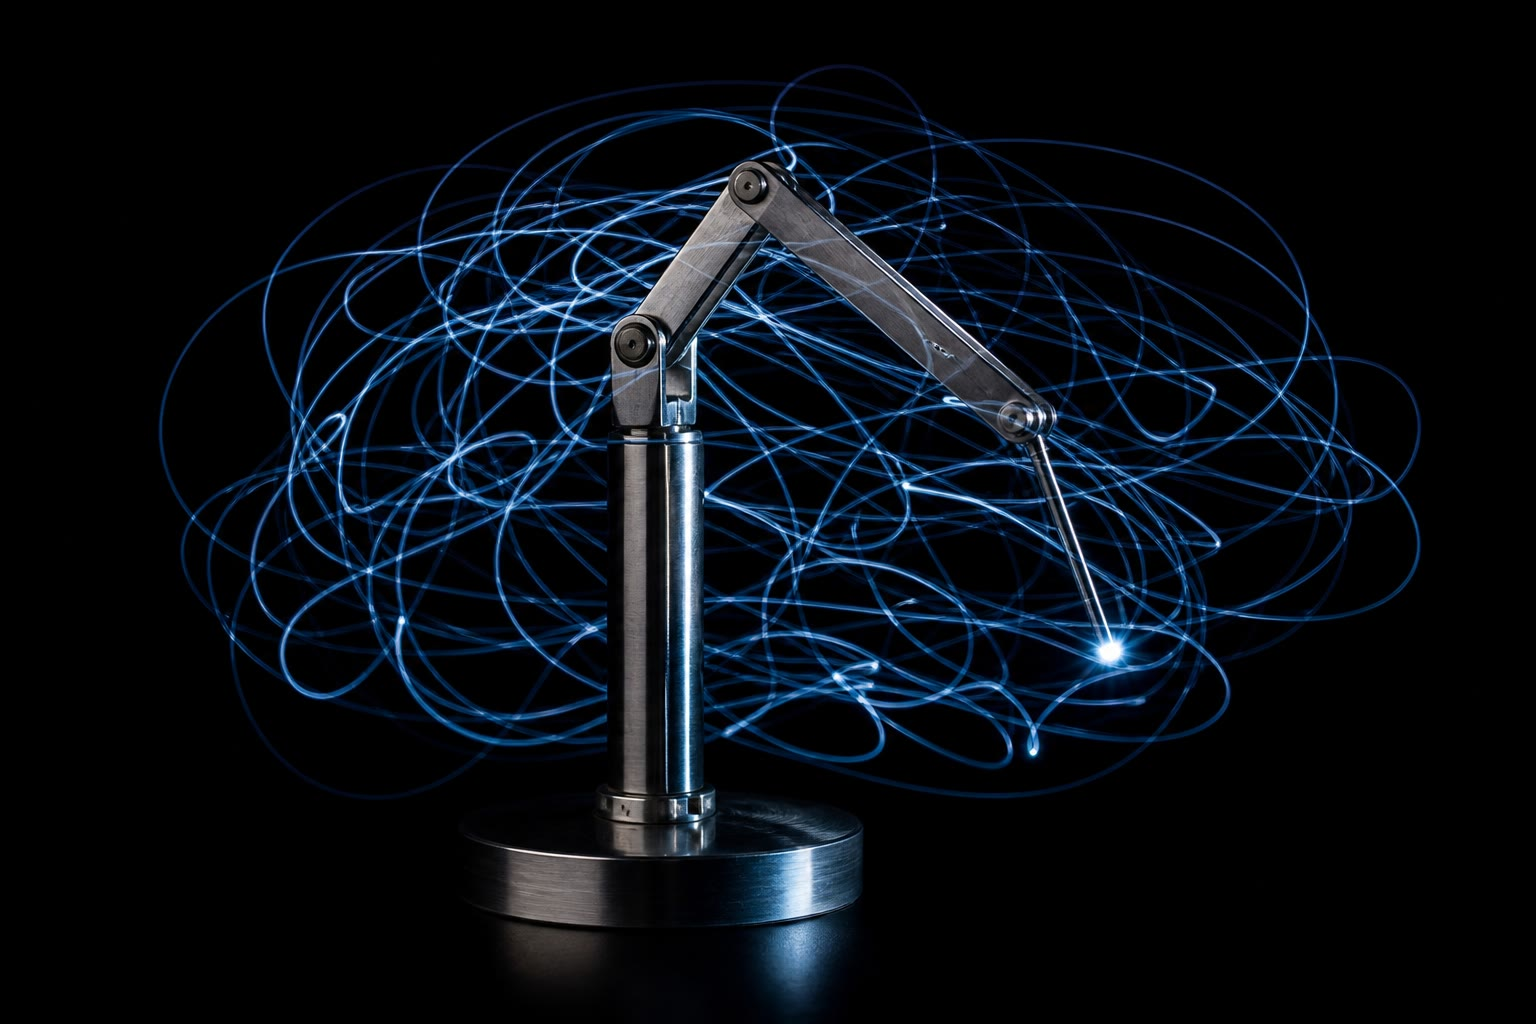
\includegraphics[width=0.58\linewidth]{images/book5/ai/b5-01-double-pendulum-trace.jpg}

{\small Een dubbele slinger vastgelegd met een lange belichtingstijd: twee coördinaten, één \omterm{def:b3:lagrangian-mechanics:action}{lagrangiaan}, en een beweging die geen formule lang vooruit voorspelt --- het apparaat van de \omterm{thm:b3:lagrangian-mechanics:euler-lagrange}{kleinste actie} uit dit hoofdstuk schrijft de vergelijkingen; de chaos houdt hun oplossingen bescheiden.}
\end{omfigure}

\section{Opgaven}

\begin{exercise}[$\star$]\label{exo:b3:lagrangian-mechanics:1}
Tel de \omterm{def:b3:lagrangian-mechanics:coordinates}{vrijheidsgraden} en stel \omterm{def:b3:lagrangian-mechanics:coordinates}{gegeneraliseerde coördinaten} voor: (a) een
deeltje aan de binnenkant van een vaste schaal; (b) een cilinder die
zonder slippen langs een vast hellend vlak rolt; (c) een dubbele slinger
waarvan het bovenste draaipunt over een horizontale rail schuift; (d) een
halter (twee massa's, starre staaf) in de ruimte; (e) twee kralen op
dezelfde vaste cirkelvormige draad. Welke \omterm{def:b3:lagrangian-mechanics:coordinates}{dwangvoorwaarde} in deze lijst
betreft snelheden in plaats van posities, en waarom is zij toch tot een
holonome te integreren?
\end{exercise}

\begin{exercise}[$\star$]\label{exo:b3:lagrangian-mechanics:2}
Voor de vlakke slinger (\cref{ex:b3:lagrangian-mechanics:pendulum}):
(a) controleer de dimensies van $L$ en van $p_\theta =
\partial L/\partial\dot\theta$; (b) benoem $p_\theta$ natuurkundig; (c)
leid de periode voor kleine hoeken af; (d) bereken de \omterm{def:b3:lagrangian-mechanics:action}{actie} $S$ van één
volledige kleine trilling met amplitude $\theta_0$ --- en verklaar het
antwoord vóór u rekent (wat is het tijdgemiddelde van $E_k - E_p$ voor
een harmonische trilling?).
\end{exercise}

\begin{exercise}[$\star$]\label{exo:b3:lagrangian-mechanics:3}
Een machine van Atwood: de massa's $m_1$ en $m_2$ hangen aan een ideaal
koord over een massaloze katrol. (a) Kies één coördinaat en schrijf $L$.
(b) Bepaal de versnelling. (c) De aanpak van Newton had de spankracht
nodig --- waar is die gebleven? (d) Hoe zou u de spankracht terugvinden
zodra de beweging bekend is?
\end{exercise}

\begin{exercise}[$\star$]\label{exo:b3:lagrangian-mechanics:4}
Een vrij deeltje in cilindercoördinaten: $L = \tfrac12 m(\dot r^2 +
r^2\dot\varphi^2 + \dot z^2)$. (a) Welke coördinaten zijn cyclisch, en
welke impulsen blijven behouden? (b) Waarom blijft $p_r$ \emph{niet}
behouden, hoewel er geen kracht werkt? (c) Schrijf de vergelijking van
Euler--Lagrange voor $r$ op en duid de term $mr\dot\varphi^2$. (d) Ga na
dat een rechte lijn met constante snelheid eraan voldoet.
\end{exercise}

\begin{exercise}[$\star\star$]\label{exo:b3:lagrangian-mechanics:5}
Een blok met massa $m$ glijdt over het wrijvingsloze vlak (hoek $\alpha$)
van een wig met massa $M$, die zelf vrij over een wrijvingsloze vloer kan
schuiven. (a) Kies twee coördinaten: de abscis $X$ van de wig en de
afstand $s$ die het blok langs het vlak heeft afgelegd; schrijf $L$.
(b) Welke coördinaat is cyclisch, en welke behoudswet drukt zij uit?
(c) Bepaal de twee versnellingen. (d) Toets de limieten $M \to \infty$ en
$\alpha \to
90^\circ$.
\end{exercise}

\begin{exercise}[$\star\star$]\label{exo:b3:lagrangian-mechanics:6}
De bolslinger: een gewicht aan een staaf met lengte $\ell$, vrij in beide
hoeken ($\theta$ vanaf de neerwaartse verticaal, $\varphi$ eromheen).
(a) Schrijf $L$. (b) Benoem de \omterm{def:b3:lagrangian-mechanics:momentum}{cyclische coördinaat} en de behouden
$p_\varphi$. (c) Herleid de beweging van $\theta$ tot een effectieve
potentiaal en schets die. (d) Vind voor de kegelbeweging $\theta =
\theta_0$ de betrekking $\cos\theta_0 =
g/\ell\omega^2$ van de
kegelslinger uit het volume van jaar 1 terug.
\end{exercise}

\begin{exercise}[$\star\star$]\label{exo:b3:lagrangian-mechanics:7}
Een slinger (massa $m$, lengte $\ell$) hangt aan een wagentje met massa
$M$ dat vrij over een horizontale rail rolt. (a) Schrijf met de
coördinaten $X$ (wagentje) en $\theta$ de \omterm{def:b3:lagrangian-mechanics:action}{lagrangiaan} $L$ op. (b) Wat
blijft behouden, en
waarom natuurkundig? (c) Lineariseer voor kleine $\theta$ en toon aan dat
de trillingsfrequentie $\Omega = \sqrt{(1 + m/M)\,g/\ell}$ bedraagt.
(d) Verklaar de limieten $M \to
\infty$ en $M \to 0$ --- waarom
\emph{verhoogt} een licht wagentje de frequentie?
\end{exercise}

\begin{exercise}[$\star\star$]\label{exo:b3:lagrangian-mechanics:8}
Een deeltje met lading $q$ in een uniform veld $\vect B = B\vect e_z$,
beschreven door $\vect A = \tfrac12\vect B\wedge\vect r$. (a) Schrijf $L$
in cartesische coördinaten. (b) Leid de bewegingsvergelijkingen af en ga
na dat zij de cyclotroncirkel bij $\omega_{\text{c}} = qB/m$ beschrijven.
(c) Bereken de geconjugeerde impulsen $p_x$ en $p_y$: zijn zij $m\dot x$
en $m\dot y$? Blijven zij behouden? (d) Toon aan dat $L$ in
cilindercoördinaten $\varphi$ cyclisch heeft, en benoem de behouden
$p_\varphi$ voor een cirkel met de as als middelpunt.
\end{exercise}

\begin{exercise}[$\star\star$]\label{exo:b3:lagrangian-mechanics:9}
Voor de kraal op de draaiende hoepel
(\cref{ex:b3:lagrangian-mechanics:hoop}): (a) bereken de \omterm{prop:b3:lagrangian-mechanics:energy}{energiefunctie}
$h$ en ga met de bewegingsvergelijking na dat zij behouden blijft;
(b) bereken de mechanische energie $E$ en toon aan dat $E - h =
m\omega^2R^2\sin^2\theta$; (c) bepaal het vermogen dat de motor levert als
functie van $\theta$ en $\dot\theta$; (d) bepaal de frequentie van \omterm{prop:b3:lagrangian-mechanics:modes}{kleine
trillingen} om het gekantelde evenwicht wanneer $\omega^2 > g/R$, en toon
aan dat zij naar nul gaat als $\omega^2 \to g/R$ --- de vertraging die de
splitsing van de put aankondigt.
\end{exercise}

\begin{exercise}[$\star\star\star$]\label{exo:b3:lagrangian-mechanics:10}
De gelijkbenige dubbele slinger ($m_1 = m_2 = m$, $\ell_1 = \ell_2 = \ell$). (a) Toon aan dat voor kleine hoeken $L = \tfrac12 m\ell^2(2\dot\theta_1^2 +
2\dot\theta_1\dot\theta_2 + \dot\theta_2^2) - \tfrac12 mg\ell(2
\theta_1^2 + \theta_2^2)$. (b) Schrijf de twee
bewegingsvergelijkingen op. (c) Bepaal de eigenfrequenties $\Omega_\pm^2 = (2 \mp \sqrt2)\,g/\ell$ en de vorm van elke modus ($\theta_2 = \pm\sqrt2\,\theta_1$). (d) Bij grote amplitude is dit stelsel een
standaardvoorbeeld van chaos: leg in enkele regels uit wat de analyse voor
kleine hoeken breekt, en waarom er geen enkele behoudswet verloren gaat.
\end{exercise}

\begin{exercise}[$\star\star\star$]\label{exo:b3:lagrangian-mechanics:11}
\emph{De brachistochroon.} Een kraal glijdt zonder wrijving vanuit rust in
de oorsprong langs een kromme $y(x)$ ($y$ naar beneden) naar een punt $(a, b)$. (a) Toon met behoud van energie aan dat de daaltijd $T =
\int_0^a\sqrt{(1 + y'^2)/2gy}\,\dd x$ bedraagt --- een functionaal, waarin
$x$ de rol van de tijd speelt. (b) De integrand $F(y, y')$ bevat geen
expliciete $x$: toon aan dat $h = y'\,\partial F/\partial y' - F$ constant
is langs de optimale kromme (dezelfde berekening als in
\cref{prop:b3:lagrangian-mechanics:energy}). (c) Leid $y(1 + y'^2) =
2r$
af voor een constante $r$, en ga na dat de cycloïde $x = r(\phi -
\sin\phi)$, $y = r(1 - \cos\phi)$ eraan voldoet. (d) Toon aan dat de kraal
er $\pi\sqrt{r/g}$ over doet om de onderkant van één boog te bereiken, en
vergelijk met de rechte glijbaan naar hetzelfde punt.
\end{exercise}

\begin{exercise}[$\star\star\star$]\label{exo:b3:lagrangian-mechanics:12}
\emph{Fermat als \omterm{thm:b3:lagrangian-mechanics:euler-lagrange}{kleinste actie}.} Licht in een middenstof met index $n(y)$
legt de weg tussen twee punten in de kortste tijd af (volume van jaar 2).
(a) Toon aan dat de looptijd langs $y(x)$ gelijk is aan $T = \tfrac1c\int n(y)\sqrt{1 +
y'^2}\,\dd x$. (b) Omdat de integrand geen
expliciete $x$ bevat, gebruikt u de behouden $h$ van de vorige opgave om
aan te tonen dat $n(y)\big/\sqrt{1 +
y'^2} = \text{const}$, en ga na dat
dit de wet van Snellius $n\sin i =
\text{const}$ is voor een straal
gemeten vanaf de verticaal. (c) Boven een heet wegdek groeit de index met
de hoogte als $n(y) \approx n_0(1 + \beta y)$; toon aan dat een bijna
horizontale straal buigt met kromtestraal $R \approx
1/\beta$. (d) Vanaf
welke afstand ziet een bestuurder met de ogen op \qty{1.2}{m} boven het
wegdek de ``waterplas'' als luchtspiegeling, met $\beta = \qty{1.2e-5}{m^{-1}}$?
\end{exercise}

\begin{omfigure}
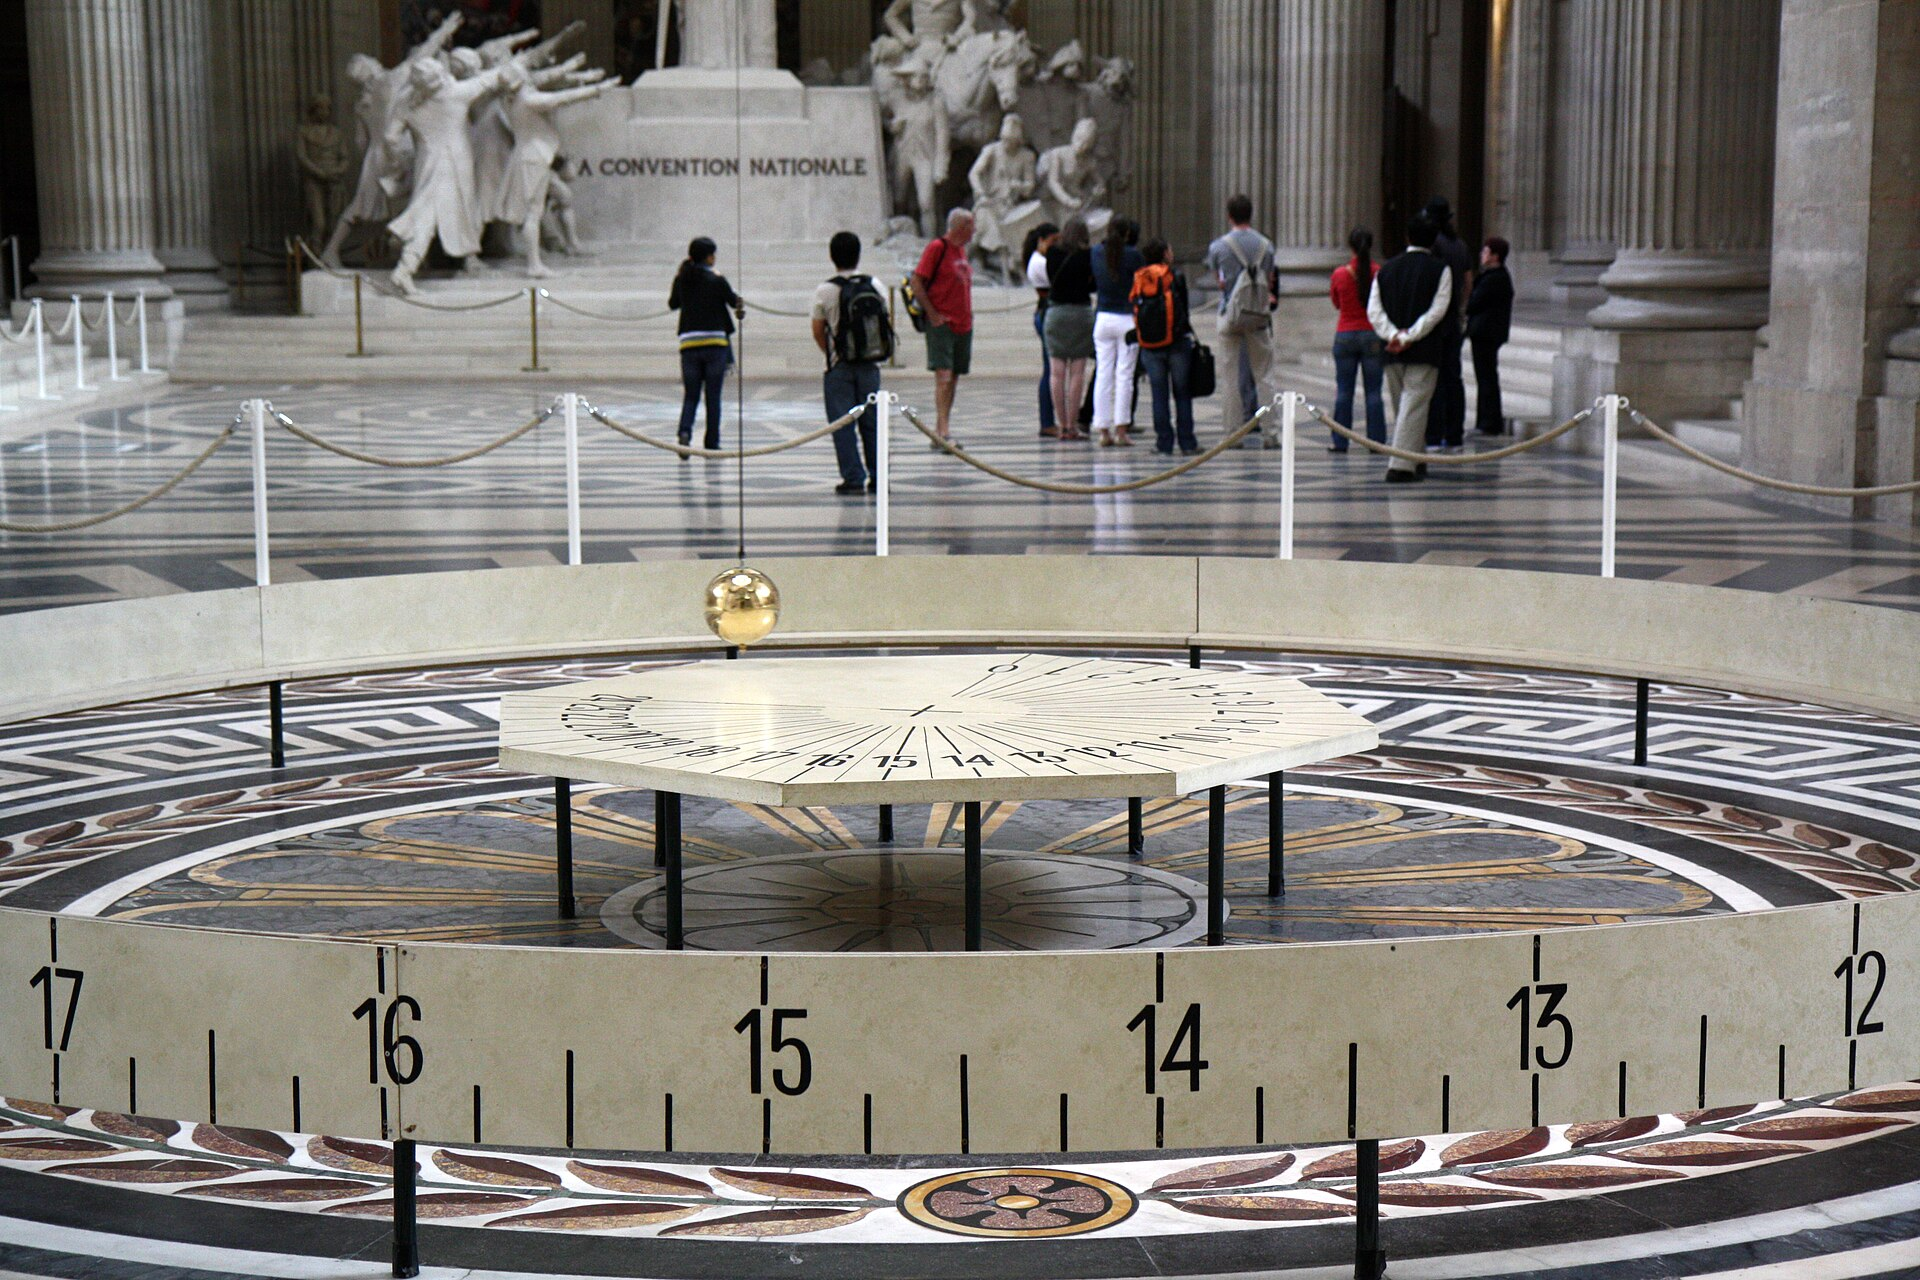
\includegraphics[width=0.6\linewidth]{images/book5/photo-foucault-pantheon.jpg}

{\small De slinger van Foucault in het Panthéon te Parijs. \omterm{def:b3:lagrangian-mechanics:coordinates}{Gegeneraliseerde coördinaten}, een \omterm{def:b3:lagrangian-mechanics:coordinates}{dwangvoorwaarde} en een langzaam draaiend assenstelsel: de rotatie van de zaal duikt op in de bewegingsvergelijkingen --- en de drift van het slingervlak laat een kelder de omwenteling van de aarde meten. Foto: Olga Khomitsevich, CC~BY~2.0.}
\end{omfigure}

\section{Vraagstuk: De bezem die op zijn kop blijft staan}

\begin{problem}[{Weekendvraagstuk --- De omgekeerde slinger van Kapitza}]\label{pb:b3:lagrangian-mechanics:1}
Een starre slinger kan stabiel \emph{boven} zijn draaipunt staan wanneer
dat draaipunt snel genoeg op en neer wordt geschud --- een verschijnsel
dat Kapitza in 1951 analyseerde, opvallend genoeg om op een goocheltruc te
lijken, en het beginsel waarmee oscillerende elektrische velden losse
ionen vangen. We modelleren de slinger als een puntmassa $m$ aan het
uiteinde van een massaloze starre staaf met lengte $\ell = \qty{40}{cm}$;
$\theta$ is de hoek vanaf de \emph{neerwaartse} verticaal en $g = \qty{9.81}{m/s^2}$.

\medskip\noindent\textbf{Deel I --- De starre slinger.}
Het draaipunt wordt eerst vastgehouden.
\begin{enumerate}
  \item Schrijf de \omterm{def:b3:lagrangian-mechanics:action}{lagrangiaan} en de bewegingsvergelijking op.
  \item Geef de frequentie $f_0$ van \omterm{prop:b3:lagrangian-mechanics:modes}{kleine trillingen} om $\theta =
        0$,
        en haar waarde.
  \item Toon aan dat hier $h = E$ geldt, en gebruik het behoud ervan om
        de minimale beginsnelheid van het gewicht onderaan te vinden die
        het tot de top brengt.
  \item Lineariseer de vergelijking nabij $\theta = \pi$ (stel $\theta = \pi +
        \epsilon$) en toon aan dat $\ddot\epsilon = +(g/\ell)\epsilon$: hoe snel groeit een aanvankelijke helling van
        een milligraad? Geef de tijd waarin zij met een factor $e$ groeit.
  \item Een bezem op een vingertop valt in ongeveer een seconde om en
        blijft toch nooit alleen staan: zeg in één zin wat de
        gelineariseerde vergelijking over het evenwicht $\theta = \pi$
        zegt.
\end{enumerate}

\medskip\noindent\textbf{Deel II --- Het draaipunt geschud.}
Het draaipunt trilt nu verticaal, met hoogte $y_{\text{s}}(t) =
a\cos\Omega t$, waarbij $a = \qty{2.0}{cm}$ en $\Omega$ instelbaar is.
\begin{enumerate}[resume]
  \item Schrijf de coördinaten van het gewicht op en toon aan dat
        $\vect v^{\,2} = \ell^2\dot\theta^2 -
        2a\Omega\ell\sin(\Omega t)\sin\theta\,\dot\theta +
        a^2\Omega^2\sin^2\Omega t$.
  \item Toon aan dat twee lagrangianen die een totale tijdsafgeleide
        $\dd F(q,t)/\dd t$ verschillen, dezelfde \omterm{thm:b3:lagrangian-mechanics:euler-lagrange}{vergelijkingen van
        Euler--Lagrange} geven.
  \item Herleid de \omterm{def:b3:lagrangian-mechanics:action}{lagrangiaan} met deze vrijheid tot $L = \tfrac12 m
        \ell^2\dot\theta^2 - ma\Omega^2\ell\cos(\Omega t)\cos\theta +
        mg\ell\cos\theta$. (Aanwijzing: $\sin(\Omega t)\sin\theta\,\dot\theta$
        vormt samen met een term $\cos(\Omega t)\cos\theta$
        een totale afgeleide; termen die alleen van $t$ afhangen mogen
        vervallen.)
  \item Leid de bewegingsvergelijking af
        \[
        \ddot\theta = -\frac{g}{\ell}\sin\theta
         + \frac{a\Omega^2}{\ell}\cos(\Omega t)\sin\theta .
        \]
        Duid de tweede term als het vervangen van de zwaartekracht door
        $g +
        \ddot y_{\text{s}}$: de slinger zit in een lift.
  \item Blijft de \omterm{prop:b3:lagrangian-mechanics:energy}{energiefunctie} $h$ nu behouden? En de energie? Wat
        pompt er energie in en uit?
  \item In het regime van Kapitza geldt $a \ll \ell$ en $\Omega \gg \omega_0 =
        \sqrt{g/\ell}$: ga dit na voor $a = \qty{2}{cm}$,
        $\ell =
        \qty{40}{cm}$ en $\Omega/2\pi = \qty{40}{Hz}$, en leg
        natuurkundig uit waarom het gewicht de aandrijving dan niet kan
        volgen.
\end{enumerate}

\medskip\noindent\textbf{Deel III --- Snel en traag gescheiden.}
Zoek de beweging als $\theta(t) = \Theta(t) + \xi(t)$: een trage drift
$\Theta$ plus een kleine rimpel $\xi$ op de aandrijffrequentie.
\begin{enumerate}[resume]
  \item Toon aan, door aan weerszijden alleen de grootste term te
        houden, dat de rimpel voldoet aan
        $\ddot\xi \approx +(a\Omega^2/\ell)\cos(\Omega t)
        \sin\Theta$, met $\Theta$
        bevroren op de tijdschaal van de aandrijving.
  \item Leid $\xi(t) = -(a/\ell)\cos(\Omega t)\sin\Theta$ af en ga na
        dat de amplitude ervan klein is, van de orde $a/\ell$.
  \item Ontwikkel $\sin\theta = \sin(\Theta + \xi)$ tot op eerste orde in
        $\xi$ en vul dit in de bewegingsvergelijking in.
  \item Middel over één aandrijfperiode, met $\Theta$ vastgehouden: toon
        met $\langle\cos\Omega t\rangle = 0$ en
        $\langle\cos^2\Omega t\rangle = \tfrac12$ aan dat
        \[
        \ddot\Theta = -\frac{g}{\ell}\sin\Theta
         - \frac{a^2\Omega^2}{2\ell^2}\sin\Theta\cos\Theta .
        \]
  \item Toon aan dat dit een beweging in de effectieve potentiaal is
        \[
        U_{\text{eff}}(\Theta) = mg\ell\Big({-\cos\Theta}
         + \frac{a^2\Omega^2}{4g\ell}\sin^2\Theta\Big) .
        \]
  \item Vergelijk met de kraal op de draaiende hoepel
        (\cref{ex:b3:lagrangian-mechanics:hoop}): dezelfde wiskunde,
        maar het tegengestelde teken van de nieuwe term --- wat doet het
        schudden met het \emph{onderste} evenwicht dat de rotatie niet
        deed?
  \item Schets $U_{\text{eff}}$ voor trage en voor snelle aandrijving, en
        beschrijf in elk geval elk evenwicht en zijn stabiliteit.
\end{enumerate}

\medskip\noindent\textbf{Deel IV --- De bezem gaat staan.}
\begin{enumerate}[resume]
  \item Ontwikkel $U_{\text{eff}}$ nabij $\Theta = \pi$ en toon aan dat
        de omgekeerde stand precies stabiel is wanneer
        \[
        a^2\Omega^2 > 2g\ell .
        \]
  \item Bereken de kritische aandrijffrequentie $f_{\text{c}} =
        \Omega_{\text{c}}/2\pi$ voor onze slinger, en de piekwaarden van
        de snelheid $a\Omega_{\text{c}}$ en de versnelling
        $a\Omega_{\text{c}}^2$ (in eenheden van $g$) die zij van het
        draaipunt eist.
  \item Bepaal bij $\Omega = 2\Omega_{\text{c}}$ de frequentie van het
        trage wiegen van de staande slinger om $\Theta = \pi$, en haar
        waarde; ga na dat zij inderdaad traag is vergeleken met de
        aandrijving.
  \item Nog steeds bij $\Omega = 2\Omega_{\text{c}}$: hoe groot is de
        rimpelamplitude $\xi$ in graden bij een $\Theta$ iets naast
        $\pi$, voor $a/\ell = 0.05$? Zou een foto de truc verraden?
  \item Hoever mag de bezem uit de verticaal hellen en toch terugkeren?
        Toon aan dat de staande put zich uitstrekt over $|\Theta - \pi| <
        \arccos(2g\ell/a^2\Omega^2)$, en evalueer dit bij $\Omega =
        2\Omega_{\text{c}}$.
  \item Een jongleur die een bezem op een stilstaande vingertop
        balanceert houdt hem ook overeind --- met welk geheel ander
        mechanisme? Noem het kenmerk van de slinger van Kapitza dat geen
        terugkoppeling nodig heeft.
  \item Vat het genoemde resultaat samen: een draaipunt dat met amplitude
        \qty{2}{cm} bij \qty{45}{Hz} wordt geschud --- tweemaal de
        kritische frequentie --- houdt een slinger van \qty{40}{cm}
        ondersteboven, in een put die tot zo'n $75^\circ$ uit de
        verticaal reikt en die zachtjes wiegt bij ongeveer
        \qty{1.4}{Hz}. Waar in de natuurkunde wordt dezelfde
        uitgemiddelde vangst gebruikt om één geladen deeltje vast te
        houden?
\end{enumerate}
\end{problem}
